\documentclass[aspectratio=169]{beamer}

% Theme and colors
\usetheme{Madrid}
\usecolortheme{default}

% Define custom colors for classes
\definecolor{classA}{RGB}{31, 119, 180}   % Blue (threads / IO-bound)
\definecolor{classB}{RGB}{255, 127, 14}   % Orange (processes / CPU-bound)
\definecolor{splitline}{RGB}{44, 160, 44} % Green for insight boxes

% Packages
\usepackage{tikz}
\usepackage{amsmath}
\usepackage{amssymb}
\usepackage{booktabs}
\usepackage{listings}
\usetikzlibrary{shapes, arrows.meta, positioning, calc, patterns, decorations.pathreplacing}

% Listings style for Python
\lstset{
    language=Python,
    basicstyle=\ttfamily\scriptsize,
    keywordstyle=\color{classA}\bfseries,
    stringstyle=\color{splitline!80!black},
    commentstyle=\color{gray},
    showstringspaces=false,
    frame=single,
    framerule=0.5pt,
    backgroundcolor=\color{gray!5},
    xleftmargin=2pt,
    xrightmargin=2pt,
    aboveskip=4pt,
    belowskip=4pt,
}

% Title information
\title{Concurrency in Python: Threads and Processes}
\subtitle{IO-Bound vs. CPU-Bound Work and the GIL}
\author{}
\date{}

\begin{document}

% -----------------------------------------------------------------------------
% Slide 1: Title
% -----------------------------------------------------------------------------
\begin{frame}
    \titlepage
\end{frame}

% -----------------------------------------------------------------------------
% Slide 2: Terminology -- Cores, Hardware Threads, Software Threads
% -----------------------------------------------------------------------------
\begin{frame}{Cores, Hardware Threads, and Software Threads}
    \begin{columns}
        \begin{column}{0.45\textwidth}
            \centering
            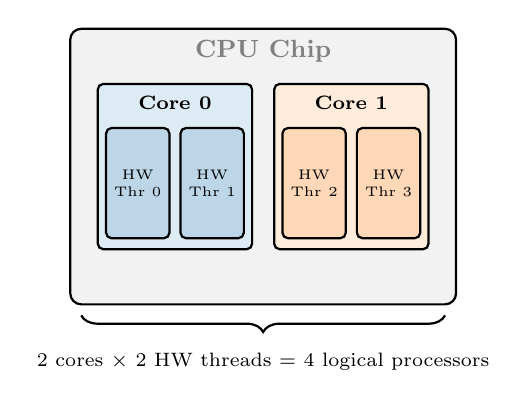
\begin{tikzpicture}[scale=0.7]
                % CPU chip outline
                \draw[thick, rounded corners=4pt, fill=gray!10] (-0.5,-0.5) rectangle (6.5,4.5);
                \node[font=\small\bfseries, gray] at (3,4.1) {CPU Chip};

                % Core 0
                \draw[thick, fill=classA!15, rounded corners=2pt] (0,0.5) rectangle (2.8,3.5);
                \node[font=\scriptsize\bfseries] at (1.4,3.15) {Core 0};
                \draw[thick, fill=classA!30, rounded corners=2pt] (0.15,0.7) rectangle (1.3,2.7);
                \node[font=\tiny, align=center] at (0.725,1.7) {HW\\Thr 0};
                \draw[thick, fill=classA!30, rounded corners=2pt] (1.5,0.7) rectangle (2.65,2.7);
                \node[font=\tiny, align=center] at (2.075,1.7) {HW\\Thr 1};

                % Core 1
                \draw[thick, fill=classB!15, rounded corners=2pt] (3.2,0.5) rectangle (6.0,3.5);
                \node[font=\scriptsize\bfseries] at (4.6,3.15) {Core 1};
                \draw[thick, fill=classB!30, rounded corners=2pt] (3.35,0.7) rectangle (4.5,2.7);
                \node[font=\tiny, align=center] at (3.925,1.7) {HW\\Thr 2};
                \draw[thick, fill=classB!30, rounded corners=2pt] (4.7,0.7) rectangle (5.85,2.7);
                \node[font=\tiny, align=center] at (5.275,1.7) {HW\\Thr 3};

                % Brace below
                \draw[decorate, decoration={brace, amplitude=6pt, mirror}, thick]
                    (-0.3,-0.7) -- (6.3,-0.7);
                \node[font=\scriptsize, below] at (3,-1.2) {2 cores $\times$ 2 HW threads = 4 logical processors};
            \end{tikzpicture}
        \end{column}
        \begin{column}{0.52\textwidth}
            \textbf{CPU Core} --- a physical processing unit on the chip.
            Each core executes instructions independently.

            \pause
            \vspace{0.6em}
            \textbf{Hardware Thread (SMT)} --- each core presents as
            2+ logical processors. When one stalls on a memory
            fetch, the other uses the execution units.

            \pause
            \vspace{0.6em}
            \textbf{Software Thread} --- an OS-scheduled sequence of
            instructions. A program can create thousands, regardless of
            hardware thread count.

            \vspace{0.8em}
            \textit{\small This presentation focuses on software threads.}
        \end{column}
    \end{columns}
\end{frame}

% -----------------------------------------------------------------------------
% Slide 3: Concurrency vs. Parallelism
% -----------------------------------------------------------------------------
\begin{frame}{Concurrency vs. Parallelism}
    \begin{columns}
        \begin{column}{0.50\textwidth}
            \centering
            % Concurrency diagram
            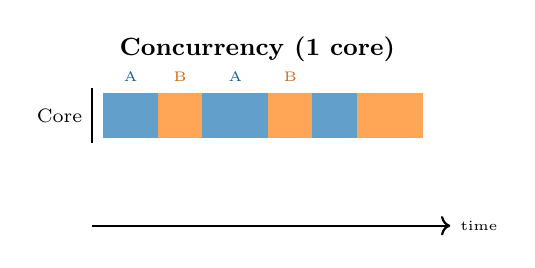
\begin{tikzpicture}[scale=0.7]
                \node[font=\small\bfseries] at (3,3.2) {Concurrency (1 core)};
                \draw[->, thick] (0,0) -- (6.5,0) node[right, font=\tiny] {time};
                \node[left, font=\scriptsize] at (0,2) {Core};
                \draw[thick] (0,1.5) -- (0,2.5);

                % Interleaved task segments
                \fill[classA!70] (0.2,1.6) rectangle (1.2,2.4);
                \fill[classB!70] (1.2,1.6) rectangle (2.0,2.4);
                \fill[classA!70] (2.0,1.6) rectangle (3.2,2.4);
                \fill[classB!70] (3.2,1.6) rectangle (4.0,2.4);
                \fill[classA!70] (4.0,1.6) rectangle (4.8,2.4);
                \fill[classB!70] (4.8,1.6) rectangle (6.0,2.4);

                \node[font=\tiny, classA!80!black] at (0.7,2.7) {A};
                \node[font=\tiny, classB!80!black] at (1.6,2.7) {B};
                \node[font=\tiny, classA!80!black] at (2.6,2.7) {A};
                \node[font=\tiny, classB!80!black] at (3.6,2.7) {B};
            \end{tikzpicture}

            \vspace{0.8em}

            % Parallelism diagram
            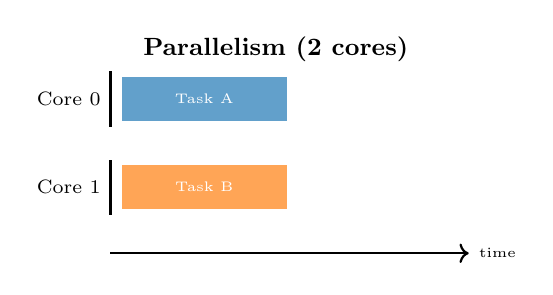
\begin{tikzpicture}[scale=0.7]
                \node[font=\small\bfseries] at (3,3.7) {Parallelism (2 cores)};
                \draw[->, thick] (0,0) -- (6.5,0) node[right, font=\tiny] {time};
                \node[left, font=\scriptsize] at (0,2.8) {Core 0};
                \node[left, font=\scriptsize] at (0,1.2) {Core 1};
                \draw[thick] (0,0.7) -- (0,1.7);
                \draw[thick] (0,2.3) -- (0,3.3);

                % Simultaneous task bars
                \fill[classA!70] (0.2,2.4) rectangle (3.2,3.2);
                \fill[classB!70] (0.2,0.8) rectangle (3.2,1.6);

                \node[font=\tiny, white] at (1.7,2.8) {Task A};
                \node[font=\tiny, white] at (1.7,1.2) {Task B};
            \end{tikzpicture}
        \end{column}
        \begin{column}{0.47\textwidth}
            \textbf{Concurrency} = managing multiple tasks with
            overlapping lifetimes.

            \vspace{0.3em}
            Tasks \textit{interleave} on one core --- only one runs
            at any instant.

            \pause
            \vspace{1em}
            \textbf{Parallelism} = executing tasks \textit{simultaneously}
            on different cores.

            \vspace{0.3em}
            Parallelism is a \textit{subset} of concurrency.

            \vspace{1em}
            \small
            \colorbox{splitline!15}{\parbox{0.9\textwidth}{
                \textbf{Key distinction:} Concurrency is about
                \textit{structure}, parallelism is about
                \textit{execution}.
            }}
        \end{column}
    \end{columns}
\end{frame}

% -----------------------------------------------------------------------------
% Slide 4: Python's Global Interpreter Lock (GIL)
% -----------------------------------------------------------------------------
\begin{frame}{Python's Global Interpreter Lock (GIL)}
    \centering
    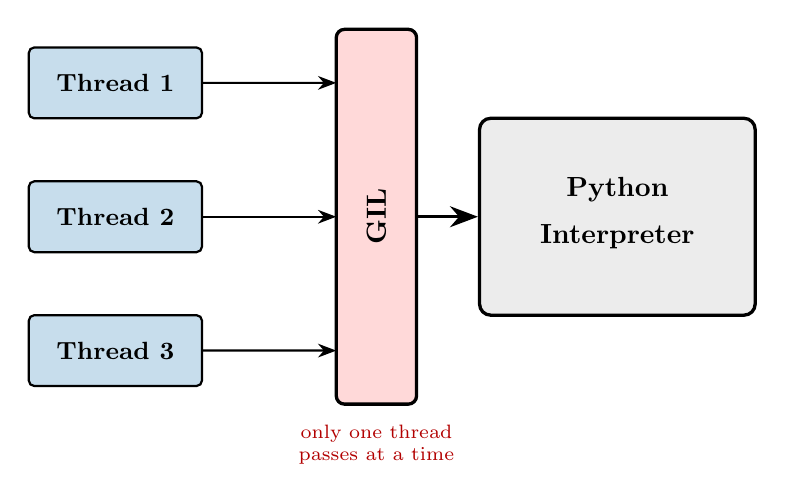
\begin{tikzpicture}[scale=0.85]
        % Thread boxes on the left
        \node[draw, thick, fill=classA!25, minimum width=2.2cm, minimum height=0.9cm,
              rounded corners=2pt, font=\small\bfseries] (t1) at (-3,2) {Thread 1};
        \node[draw, thick, fill=classA!25, minimum width=2.2cm, minimum height=0.9cm,
              rounded corners=2pt, font=\small\bfseries] (t2) at (-3,0) {Thread 2};
        \node[draw, thick, fill=classA!25, minimum width=2.2cm, minimum height=0.9cm,
              rounded corners=2pt, font=\small\bfseries] (t3) at (-3,-2) {Thread 3};

        % GIL gateway (narrow)
        \draw[very thick, fill=red!15, rounded corners=3pt] (0.3,-2.8) rectangle (1.5,2.8);
        \node[font=\bfseries, rotate=90] at (0.9,0) {GIL};

        % Arrows from threads to GIL
        \draw[-{Stealth[scale=1]}, thick] (t1.east) -- (0.3,2);
        \draw[-{Stealth[scale=1]}, thick] (t2.east) -- (0.3,0);
        \draw[-{Stealth[scale=1]}, thick] (t3.east) -- (0.3,-2);

        % Python Interpreter box on the right
        \node[draw, very thick, fill=gray!15, minimum width=3.5cm, minimum height=2.5cm,
              rounded corners=4pt] (interp) at (4.5,0) {};
        \node[font=\bfseries] at (4.5,0.4) {Python};
        \node[font=\bfseries] at (4.5,-0.3) {Interpreter};

        % Arrow from GIL to interpreter
        \draw[-{Stealth[scale=1.2]}, very thick] (1.5,0) -- (interp.west);

        % "One at a time" label
        \node[font=\scriptsize, align=center, text=red!70!black] at (0.9,-3.4)
            {only one thread\\passes at a time};
    \end{tikzpicture}

    \pause
    \vspace{0.5em}
    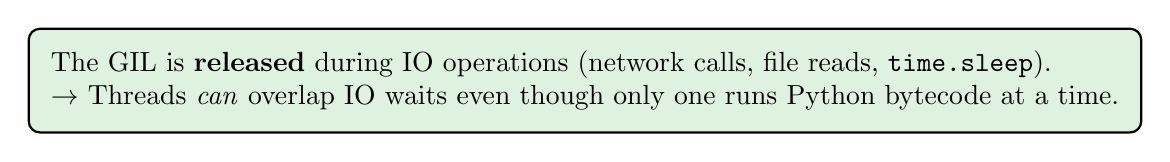
\begin{tikzpicture}
        \node[draw, thick, rounded corners, fill=splitline!15, inner sep=8pt, align=left] {
            The GIL is \textbf{released} during IO operations (network calls,
            file reads, \texttt{time.sleep}).\\
            $\rightarrow$ Threads \textit{can} overlap IO waits even though only one runs Python bytecode at a time.
        };
    \end{tikzpicture}
\end{frame}

% -----------------------------------------------------------------------------
% Slide 5: Two Approaches -- Threads vs. Processes
% -----------------------------------------------------------------------------
\begin{frame}{Two Approaches: Threads vs. Processes}
    \centering
    \small
    \begin{tabular}{lcc}
        \toprule
         & \textbf{\textcolor{classA}{Threads}} & \textbf{\textcolor{classB}{Processes}} \\
        \midrule
        Mechanism & Shared memory & Separate interpreters \\
        GIL impact & One thread runs Python at a time & Each process has its own GIL \\
        Data sharing & Direct (same address space) & Serialized (pickled) \\
        Startup cost & Lightweight & Heavier \\
        Best for & IO-bound tasks & CPU-bound tasks \\
        \bottomrule
    \end{tabular}

    \pause
    \vspace{0.8em}
    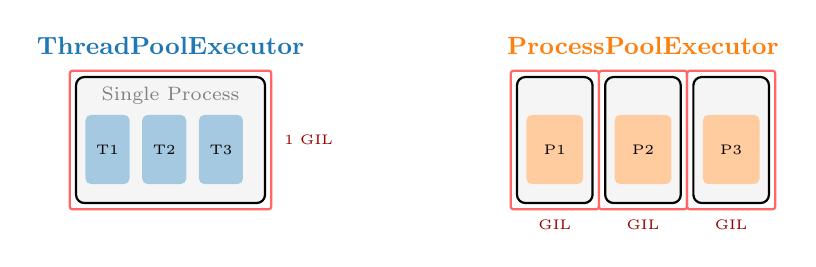
\begin{tikzpicture}[scale=0.8]
        % Threads diagram
        \begin{scope}[shift={(-4.5,0)}]
            \node[font=\small\bfseries] at (1.5,2.2) {\textcolor{classA}{ThreadPoolExecutor}};
            \draw[thick, rounded corners=3pt, fill=gray!8] (0,-0.3) rectangle (3,1.7);
            \node[font=\scriptsize, gray] at (1.5,1.4) {Single Process};
            \fill[classA!40, rounded corners=2pt] (0.15,0.0) rectangle (0.85,1.1);
            \node[font=\tiny] at (0.5,0.55) {T1};
            \fill[classA!40, rounded corners=2pt] (1.05,0.0) rectangle (1.75,1.1);
            \node[font=\tiny] at (1.4,0.55) {T2};
            \fill[classA!40, rounded corners=2pt] (1.95,0.0) rectangle (2.65,1.1);
            \node[font=\tiny] at (2.3,0.55) {T3};
            \draw[thick, red!60, rounded corners=1pt] (-0.1,-0.4) rectangle (3.1,1.8);
            \node[font=\tiny, red!60!black, right] at (3.15,0.7) {1 GIL};
        \end{scope}

        % Processes diagram
        \begin{scope}[shift={(2.5,0)}]
            \node[font=\small\bfseries] at (2,2.2) {\textcolor{classB}{ProcessPoolExecutor}};
            \foreach \i/\xoff in {1/0, 2/1.4, 3/2.8} {
                \draw[thick, rounded corners=3pt, fill=gray!8]
                    (\xoff,-0.3) rectangle (\xoff+1.2,1.7);
                \fill[classB!40, rounded corners=2pt]
                    (\xoff+0.15,0.0) rectangle (\xoff+1.05,1.1);
                \node[font=\tiny] at (\xoff+0.6,0.55) {P\i};
                \draw[thick, red!60, rounded corners=1pt]
                    (\xoff-0.1,-0.4) rectangle (\xoff+1.3,1.8);
                \node[font=\tiny, red!60!black] at (\xoff+0.6,-0.65) {GIL};
            }
        \end{scope}
    \end{tikzpicture}
\end{frame}

% -----------------------------------------------------------------------------
% Slide 6: IO-Bound Tasks -- Sequential Execution
% -----------------------------------------------------------------------------
\begin{frame}{IO-Bound Tasks: Sequential Execution}
    \begin{columns}
        \begin{column}{0.55\textwidth}
            \centering
            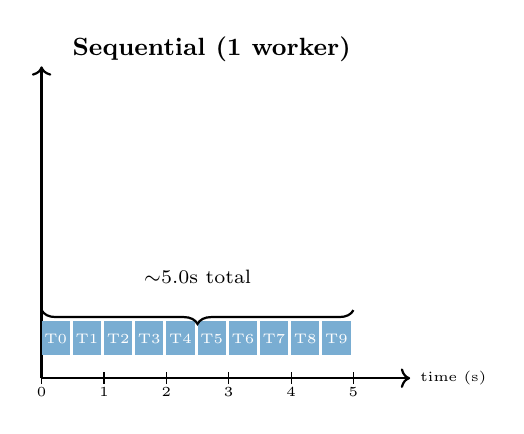
\begin{tikzpicture}[scale=0.72]
                \node[font=\small\bfseries] at (3,5.8) {Sequential (1 worker)};
                \draw[->, thick] (0,0) -- (6.5,0) node[right, font=\tiny] {time (s)};
                \draw[->, thick] (0,0) -- (0,5.5) node[above, font=\tiny] {};

                % Time axis labels
                \foreach \t in {0,1,2,3,4,5} {
                    \draw ({\t*1.1},0.1) -- ({\t*1.1},-0.1);
                    \node[below, font=\tiny] at ({\t*1.1},0) {\t};
                }

                % Sequential task bars (each 0.5s = 0.55 units)
                \foreach \i/\label in {0/T0, 1/T1, 2/T2, 3/T3, 4/T4,
                                       5/T5, 6/T6, 7/T7, 8/T8, 9/T9} {
                    \fill[classA!60] ({\i*0.55},0.4) rectangle ({\i*0.55+0.5},1.0);
                    \node[font=\tiny, white] at ({\i*0.55+0.25},0.7) {\label};
                }

                % Brace for total time
                \draw[decorate, decoration={brace, amplitude=5pt}, thick]
                    (5.5,1.2) -- (0,1.2);
                \node[font=\scriptsize, above] at (2.75,1.5) {$\sim$5.0s total};
            \end{tikzpicture}
        \end{column}
        \begin{column}{0.42\textwidth}
            A task is \textbf{IO-bound} when it spends most time
            \textit{waiting} for external resources.

            \vspace{0.5em}
            \textbf{Examples:}
            \begin{itemize}
                \item API calls
                \item File reads / writes
                \item Database queries
            \end{itemize}

            \vspace{0.5em}
            Here: 10 tasks, each taking 0.5s.

            \vspace{0.3em}
            Sequential total: $10 \times 0.5 = $ \textbf{5.0s}

            \vspace{0.3em}
            \small\textit{Each task waits for the previous one to finish.}
        \end{column}
    \end{columns}
\end{frame}

% -----------------------------------------------------------------------------
% Slide 7: IO-Bound Tasks -- ThreadPoolExecutor
% -----------------------------------------------------------------------------
\begin{frame}[fragile]{IO-Bound Tasks: ThreadPoolExecutor}
    \begin{columns}
        \begin{column}{0.55\textwidth}
            \centering
            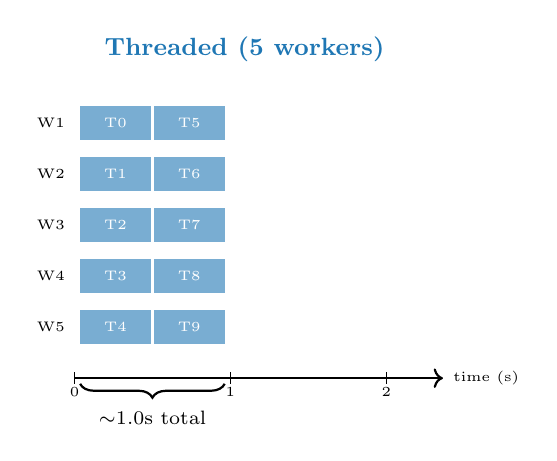
\begin{tikzpicture}[scale=0.72]
                \node[font=\small\bfseries] at (3,5.8)
                    {\textcolor{classA}{Threaded (5 workers)}};
                \draw[->, thick] (0,0) -- (6.5,0) node[right, font=\tiny] {time (s)};

                % Time axis labels
                \foreach \t in {0,1,2} {
                    \draw ({\t*2.75},0.1) -- ({\t*2.75},-0.1);
                    \node[below, font=\tiny] at ({\t*2.75},0) {\t};
                }

                % Worker lane labels
                \foreach \w/\y in {1/4.5, 2/3.6, 3/2.7, 4/1.8, 5/0.9} {
                    \node[left, font=\tiny] at (0,\y) {W\w};
                }

                % Batch 1 (0s--0.5s): 5 tasks in parallel
                \foreach \w/\y/\label in {1/4.2/T0, 2/3.3/T1, 3/2.4/T2, 4/1.5/T3, 5/0.6/T4} {
                    \fill[classA!60] (0.1,\y) rectangle (1.35,{\y+0.6});
                    \node[font=\tiny, white] at (0.725,{\y+0.3}) {\label};
                }

                % Batch 2 (0.5s--1.0s): 5 more tasks
                \foreach \w/\y/\label in {1/4.2/T5, 2/3.3/T6, 3/2.4/T7, 4/1.5/T8, 5/0.6/T9} {
                    \fill[classA!60] (1.4,\y) rectangle (2.65,{\y+0.6});
                    \node[font=\tiny, white] at (2.025,{\y+0.3}) {\label};
                }

                % Brace for total time
                \draw[decorate, decoration={brace, amplitude=5pt, mirror}, thick]
                    (0.1,-0.1) -- (2.65,-0.1);
                \node[font=\scriptsize, below] at (1.375,-0.4) {$\sim$1.0s total};
            \end{tikzpicture}
        \end{column}
        \begin{column}{0.42\textwidth}
\begin{lstlisting}[gobble=0]
with ThreadPoolExecutor(
    max_workers=5,
) as executor:
    results = executor.map(
        simulate_io_task,
        range(10),
    )
\end{lstlisting}

            \vspace{0.3em}
            GIL is \textbf{released} during \texttt{sleep()} and real IO.

            \vspace{0.3em}
            5 workers $\times$ 2 batches $=$ \textbf{$\sim$1.0s}

            \vspace{0.5em}
            \colorbox{classA!15}{\parbox{0.85\textwidth}{\centering
                \textbf{5$\times$ speedup}
            }}
        \end{column}
    \end{columns}
\end{frame}

% -----------------------------------------------------------------------------
% Slide 8: CPU-Bound Tasks -- Threads Don't Help
% -----------------------------------------------------------------------------
\begin{frame}{CPU-Bound Tasks: Threads Don't Help}
    \begin{columns}
        \begin{column}{0.50\textwidth}
            \centering
            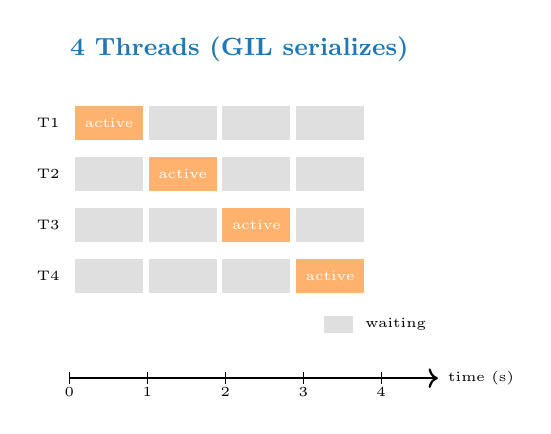
\begin{tikzpicture}[scale=0.72]
                \node[font=\small\bfseries] at (3,5.8)
                    {\textcolor{classA}{4 Threads (GIL serializes)}};
                \draw[->, thick] (0,0) -- (6.5,0) node[right, font=\tiny] {time (s)};

                % Time axis labels
                \foreach \t in {0,1,2,3,4} {
                    \draw ({\t*1.375},0.1) -- ({\t*1.375},-0.1);
                    \node[below, font=\tiny] at ({\t*1.375},0) {\t};
                }

                % Thread lane labels
                \foreach \w/\y in {1/4.5, 2/3.6, 3/2.7, 4/1.8} {
                    \node[left, font=\tiny] at (0,\y) {T\w};
                }

                % Only one thread active at a time -- serialized
                % Task 1: Thread 1 active, others waiting
                \fill[classB!60] (0.1,4.2) rectangle (1.3,4.8);
                \node[font=\tiny, white] at (0.7,4.5) {active};
                \fill[gray!25] (0.1,3.3) rectangle (1.3,3.9);
                \fill[gray!25] (0.1,2.4) rectangle (1.3,3.0);
                \fill[gray!25] (0.1,1.5) rectangle (1.3,2.1);

                % Task 2: Thread 2 active
                \fill[gray!25] (1.4,4.2) rectangle (2.6,4.8);
                \fill[classB!60] (1.4,3.3) rectangle (2.6,3.9);
                \node[font=\tiny, white] at (2.0,3.6) {active};
                \fill[gray!25] (1.4,2.4) rectangle (2.6,3.0);
                \fill[gray!25] (1.4,1.5) rectangle (2.6,2.1);

                % Task 3: Thread 3 active
                \fill[gray!25] (2.7,4.2) rectangle (3.9,4.8);
                \fill[gray!25] (2.7,3.3) rectangle (3.9,3.9);
                \fill[classB!60] (2.7,2.4) rectangle (3.9,3.0);
                \node[font=\tiny, white] at (3.3,2.7) {active};
                \fill[gray!25] (2.7,1.5) rectangle (3.9,2.1);

                % Task 4: Thread 4 active
                \fill[gray!25] (4.0,4.2) rectangle (5.2,4.8);
                \fill[gray!25] (4.0,3.3) rectangle (5.2,3.9);
                \fill[gray!25] (4.0,2.4) rectangle (5.2,3.0);
                \fill[classB!60] (4.0,1.5) rectangle (5.2,2.1);
                \node[font=\tiny, white] at (4.6,1.8) {active};

                % Gray = waiting legend
                \fill[gray!25] (4.5,0.8) rectangle (5.0,1.1);
                \node[right, font=\tiny] at (5.05,0.95) {waiting};
            \end{tikzpicture}
        \end{column}
        \begin{column}{0.47\textwidth}
            \textbf{CPU-bound:} task spends time \textit{computing},
            not waiting.

            \vspace{0.5em}
            \small
            \begin{tabular}{lc}
                \toprule
                Method & Time \\
                \midrule
                Sequential & $\sim$4s \\
                4 Threads  & $\sim$4s \\
                \bottomrule
            \end{tabular}

            \vspace{0.3em}
            \textbf{Speedup: 1.0$\times$} (no improvement)

            \pause
            \vspace{0.5em}
            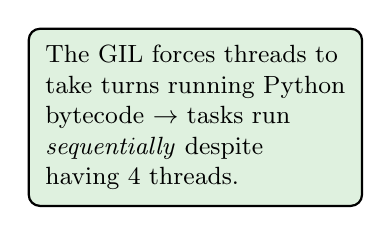
\begin{tikzpicture}
                \node[draw, thick, rounded corners, fill=splitline!15,
                      inner sep=6pt, align=left, font=\small] {
                    The GIL forces threads to\\
                    take turns running Python\\
                    bytecode $\rightarrow$ tasks run\\
                    \textit{sequentially} despite\\
                    having 4 threads.
                };
            \end{tikzpicture}
        \end{column}
    \end{columns}
\end{frame}

% -----------------------------------------------------------------------------
% Slide 9: CPU-Bound Tasks -- ProcessPoolExecutor
% -----------------------------------------------------------------------------
\begin{frame}[fragile]{CPU-Bound Tasks: ProcessPoolExecutor}
    \begin{columns}
        \begin{column}{0.55\textwidth}
            \centering
            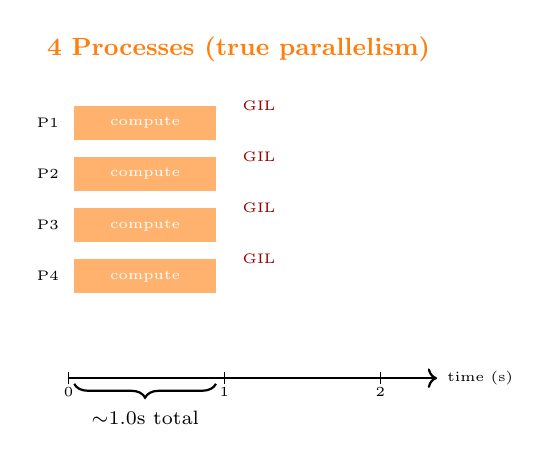
\begin{tikzpicture}[scale=0.72]
                \node[font=\small\bfseries] at (3,5.8)
                    {\textcolor{classB}{4 Processes (true parallelism)}};
                \draw[->, thick] (0,0) -- (6.5,0) node[right, font=\tiny] {time (s)};

                % Time axis labels
                \foreach \t in {0,1,2} {
                    \draw ({\t*2.75},0.1) -- ({\t*2.75},-0.1);
                    \node[below, font=\tiny] at ({\t*2.75},0) {\t};
                }

                % Process lane labels with GIL annotations
                \foreach \w/\y in {1/4.5, 2/3.6, 3/2.7, 4/1.8} {
                    \node[left, font=\tiny] at (0,\y) {P\w};
                    \node[right, font=\tiny, red!60!black] at (2.9,{\y+0.3}) {\tiny GIL};
                }

                % All 4 processes running simultaneously
                \fill[classB!60] (0.1,4.2) rectangle (2.6,4.8);
                \node[font=\tiny, white] at (1.35,4.5) {compute};
                \fill[classB!60] (0.1,3.3) rectangle (2.6,3.9);
                \node[font=\tiny, white] at (1.35,3.6) {compute};
                \fill[classB!60] (0.1,2.4) rectangle (2.6,3.0);
                \node[font=\tiny, white] at (1.35,2.7) {compute};
                \fill[classB!60] (0.1,1.5) rectangle (2.6,2.1);
                \node[font=\tiny, white] at (1.35,1.8) {compute};

                % Brace for total time
                \draw[decorate, decoration={brace, amplitude=5pt, mirror}, thick]
                    (0.1,-0.1) -- (2.6,-0.1);
                \node[font=\scriptsize, below] at (1.35,-0.4) {$\sim$1.0s total};
            \end{tikzpicture}
        \end{column}
        \begin{column}{0.42\textwidth}
\begin{lstlisting}[gobble=0]
with ProcessPoolExecutor(
    max_workers=4,
) as executor:
    results = executor.map(
        is_prime,
        numbers,
    )
\end{lstlisting}

            \vspace{0.3em}
            Same API --- just swap the class name.

            \vspace{0.3em}
            Each process has \textbf{its own GIL} $\rightarrow$ true parallel execution.

            \vspace{0.5em}
            \colorbox{classB!15}{\parbox{0.85\textwidth}{\centering
                \textbf{$\sim$4$\times$ speedup}
            }}
        \end{column}
    \end{columns}
\end{frame}

% -----------------------------------------------------------------------------
% Slide 10: Summary Speedup Comparison
% -----------------------------------------------------------------------------
\begin{frame}{Summary: Speedup Comparison}
    \centering
    \small
    \begin{tabular}{llcc}
        \toprule
        Task Type & Method & Approx. Time & Speedup \\
        \midrule
        IO-Bound (10 tasks) & Sequential & 5.0s & 1.0$\times$ \\
        IO-Bound             & \textcolor{classA}{\textbf{Threads (5 workers)}} & 1.0s
                             & \textcolor{classA}{\textbf{5.0$\times$}} \\
        IO-Bound             & Processes (5 workers) & 1.2s & 4.2$\times$ \\
        \midrule
        CPU-Bound (8 tasks) & Sequential & 4.0s & 1.0$\times$ \\
        CPU-Bound            & Threads (4 workers) & 4.0s & 1.0$\times$ \\
        CPU-Bound            & \textcolor{classB}{\textbf{Processes (4 workers)}} & 1.0s
                             & \textcolor{classB}{\textbf{4.0$\times$}} \\
        \bottomrule
    \end{tabular}

    \pause
    \vspace{0.6em}
    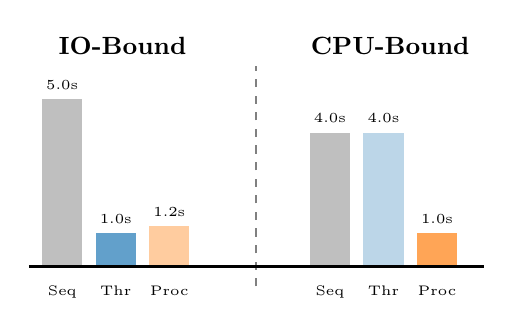
\begin{tikzpicture}[scale=0.85]
        % IO-Bound group
        \node[font=\small\bfseries] at (1.2,3.3) {IO-Bound};
        % Bars: Sequential, Threads, Processes
        \fill[gray!50] (0,0) rectangle (0.6,2.5);
        \node[font=\tiny, above] at (0.3,2.5) {5.0s};
        \node[font=\tiny, below] at (0.3,-0.15) {Seq};

        \fill[classA!70] (0.8,0) rectangle (1.4,0.5);
        \node[font=\tiny, above] at (1.1,0.5) {1.0s};
        \node[font=\tiny, below] at (1.1,-0.15) {Thr};

        \fill[classB!40] (1.6,0) rectangle (2.2,0.6);
        \node[font=\tiny, above] at (1.9,0.6) {1.2s};
        \node[font=\tiny, below] at (1.9,-0.15) {Proc};

        % Divider
        \draw[thick, dashed, gray] (3.2,-0.3) -- (3.2,3.0);

        % CPU-Bound group
        \node[font=\small\bfseries] at (5.2,3.3) {CPU-Bound};

        \fill[gray!50] (4,0) rectangle (4.6,2.0);
        \node[font=\tiny, above] at (4.3,2.0) {4.0s};
        \node[font=\tiny, below] at (4.3,-0.15) {Seq};

        \fill[classA!30] (4.8,0) rectangle (5.4,2.0);
        \node[font=\tiny, above] at (5.1,2.0) {4.0s};
        \node[font=\tiny, below] at (5.1,-0.15) {Thr};

        \fill[classB!70] (5.6,0) rectangle (6.2,0.5);
        \node[font=\tiny, above] at (5.9,0.5) {1.0s};
        \node[font=\tiny, below] at (5.9,-0.15) {Proc};

        % Axis
        \draw[thick] (-0.2,0) -- (6.6,0);
    \end{tikzpicture}
\end{frame}

% -----------------------------------------------------------------------------
% Slide 11: Decision Guide -- Threads or Processes?
% -----------------------------------------------------------------------------
\begin{frame}{Decision Guide: Threads or Processes?}
    \centering
    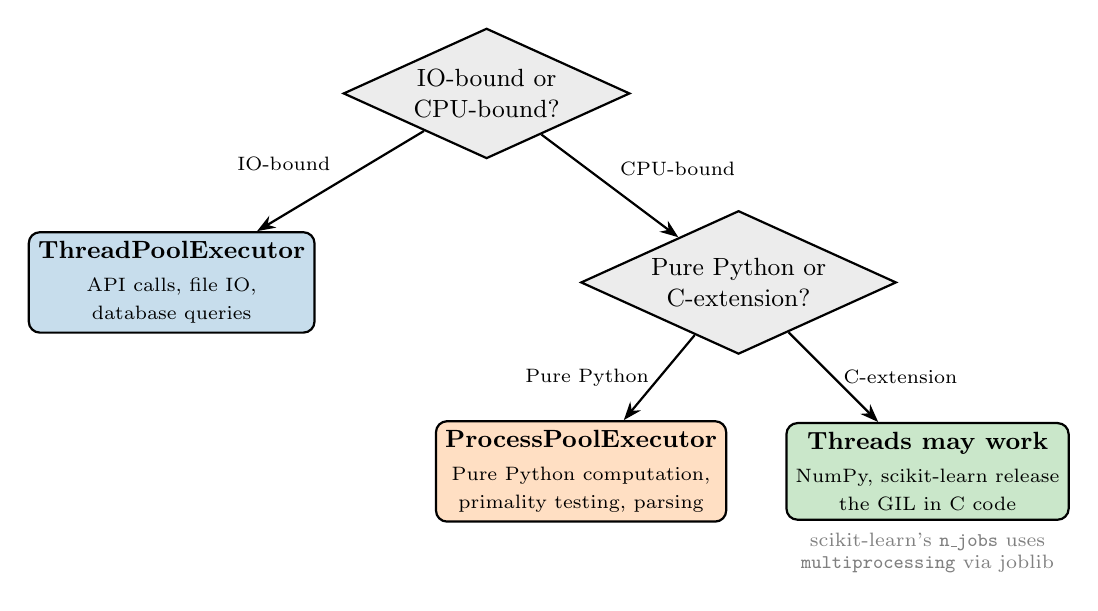
\begin{tikzpicture}[
        scale=0.8,
        decision/.style={diamond, draw, thick, fill=gray!15, inner sep=2pt,
                         align=center, font=\small, aspect=2.2},
        result/.style={rectangle, draw, thick, rounded corners=4pt,
                       minimum width=2.5cm, minimum height=1cm, align=center, font=\small},
        arrow/.style={-{Stealth[scale=1]}, thick}
    ]
        % Top decision
        \node[decision] (q1) at (0,3) {IO-bound or\\CPU-bound?};

        % IO branch
        \node[result, fill=classA!25] (io) at (-5,0)
            {\textbf{ThreadPoolExecutor}\\[0.1em]
             \scriptsize API calls, file IO,\\[-0.1em]
             \scriptsize database queries};
        \draw[arrow] (q1) -- node[above left, font=\scriptsize] {IO-bound} (io);

        % CPU branch to second decision
        \node[decision] (q2) at (4,0) {Pure Python or\\C-extension?};
        \draw[arrow] (q1) -- node[above right, font=\scriptsize] {CPU-bound} (q2);

        % Pure Python -> Processes
        \node[result, fill=classB!25] (cpu) at (1.5,-3)
            {\textbf{ProcessPoolExecutor}\\[0.1em]
             \scriptsize Pure Python computation,\\[-0.1em]
             \scriptsize primality testing, parsing};
        \draw[arrow] (q2) -- node[left, font=\scriptsize] {Pure Python} (cpu);

        % C-extension -> Threads may work
        \node[result, fill=splitline!25] (cext) at (7,-3)
            {\textbf{Threads may work}\\[0.1em]
             \scriptsize NumPy, scikit-learn release\\[-0.1em]
             \scriptsize the GIL in C code};
        \draw[arrow] (q2) -- node[right, font=\scriptsize] {C-extension} (cext);

        % Note about n_jobs
        \node[font=\scriptsize, gray, align=center] at (7,-4.3)
            {scikit-learn's \texttt{n\_jobs} uses\\
             \texttt{multiprocessing} via joblib};
    \end{tikzpicture}
\end{frame}

% -----------------------------------------------------------------------------
% Slide 12: Key Takeaways
% -----------------------------------------------------------------------------
\begin{frame}{Key Takeaways}
    \centering
    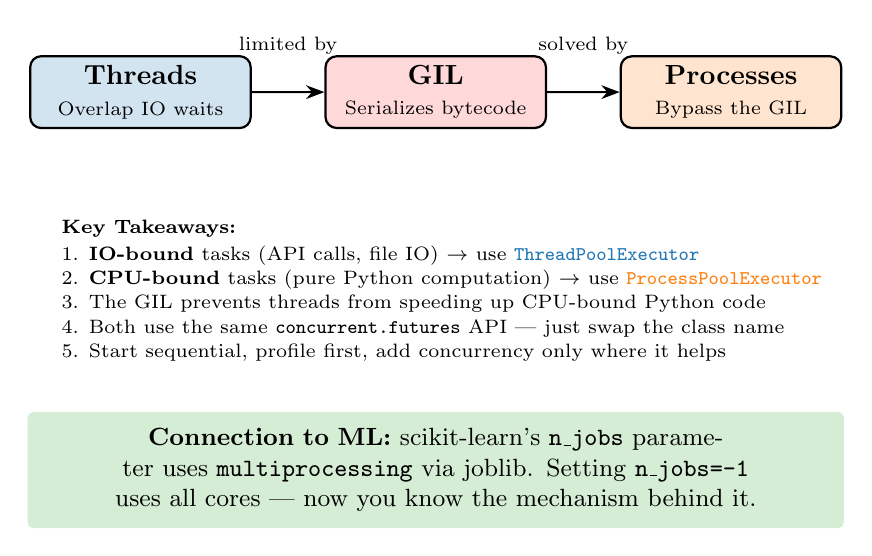
\begin{tikzpicture}[
        scale=0.75,
        box/.style={draw, thick, rounded corners, minimum width=2.8cm,
                    minimum height=0.9cm, align=center},
        arrow/.style={-{Stealth[scale=1]}, thick}
    ]
        % Three concept boxes
        \node[box, fill=classA!20] (threads) at (-5,3.2)
            {\textbf{Threads}\\[-0.1em]\scriptsize Overlap IO waits};
        \node[box, fill=red!15] (gil) at (0,3.2)
            {\textbf{GIL}\\[-0.1em]\scriptsize Serializes bytecode};
        \node[box, fill=classB!20] (procs) at (5,3.2)
            {\textbf{Processes}\\[-0.1em]\scriptsize Bypass the GIL};

        % Arrows
        \draw[arrow] (threads) -- (gil)
            node[midway, above, yshift=10pt, font=\scriptsize] {limited by};
        \draw[arrow] (gil) -- (procs)
            node[midway, above, yshift=10pt, font=\scriptsize] {solved by};

        % Key takeaways list
        \node[align=left, anchor=north west, font=\scriptsize] at (-6.5,1.2) {
            \textbf{Key Takeaways:}\\[0.2em]
            1. \textbf{IO-bound} tasks (API calls, file IO)
               $\rightarrow$ use \texttt{\textcolor{classA}{ThreadPoolExecutor}}\\[0.1em]
            2. \textbf{CPU-bound} tasks (pure Python computation)
               $\rightarrow$ use \texttt{\textcolor{classB}{ProcessPoolExecutor}}\\[0.1em]
            3. The GIL prevents threads from speeding up CPU-bound Python code\\[0.1em]
            4. Both use the same \texttt{concurrent.futures} API --- just swap the class name\\[0.1em]
            5. Start sequential, profile first, add concurrency only where it helps
        };

        % Connection box inside tikzpicture to control placement
        \node[fill=splitline!20, rounded corners=2pt, inner sep=6pt,
              align=center, font=\small,
              text width=0.82\textwidth] at (0,-3.2) {
            \textbf{Connection to ML:} scikit-learn's \texttt{n\_jobs} parameter uses
            \texttt{multiprocessing} via joblib.
            Setting \texttt{n\_jobs=-1} uses all cores --- now you know the mechanism behind it.
        };
    \end{tikzpicture}
\end{frame}

\end{document}
